\documentclass[t]{beamer}

% Load general definitions
% Preamble file - general definitions, package loading, etc.

%=================================
% Load packages
\usepackage{amssymb,amsmath}
\usepackage{graphicx}
\usepackage{url}
\usepackage{tikz}
\usetikzlibrary{mindmap,trees,arrows}
\usepackage{fancyvrb}
\usepackage[english]{babel}
\usepackage[latin1]{inputenc}
\usepackage{subfigure}
\usepackage{times}
\usepackage[T1]{fontenc}
\usepackage{cancel}
\usepackage{color}
\usepackage{listings}

%=================================
% Set mode
\mode<presentation>
{
	\usetheme{Madrid}
	\usecolortheme{whale}
	\useoutertheme{infolines}
	\setbeamercovered{invisible}
}

% Get rid of nav bar
\beamertemplatenavigationsymbolsempty

% Insert frame number at bottom of the page.
\usefoottemplate{\hfil\tiny{\color{black!90}\insertframenumber}} 

%=================================
% Define new commands

\newcommand\Real{{\mathbb{R}}}
%\newcommand{\vi}{\vspace{0.6\baselineskip}}
%\newcommand{\goodgap}{\hspace{\subfigtopskip}\hspace{\subfigbottomskip}}


% Equation environments
\newcommand{\beq}{\begin{equation}}
\newcommand{\eq}{\end{equation}}
\newcommand{\beqs}{\begin{equation*}}
\newcommand{\eqs}{\end{equation*}}
\newcommand{\beqn}{\begin{eqnarray}}
\newcommand{\eqn}{\end{eqnarray}}

% Bold variables
\newcommand{\mbf}[1]{\ensuremath{\mathbf{#1}}}

% Itemization
\newcommand{\bitem}{\begin{itemize}}
\newcommand{\eitem}{\end{itemize}}
\newcommand{\spitem}{\vskip 1em\item}
\newcommand{\bitems}{\begin{itemize}\item}
\newcommand{\benums}{\begin{enumerate}\item}
\newcommand{\eenum}{\end{enumerate}}

% color blocks
\newenvironment{colorblock}[2]{%
\setbeamercolor{block title}{#2}
\begin{block}{#1}}{\end{block}}

% Vertical spacing
\newcommand{\vone}{\vskip 1em}
\newcommand{\vhalf}{\vskip .5em}

% Frame environments
\newenvironment{ftst}[3][t]{%
\begin{frame}{environment=ftst,#1}
\frametitle{#2}
\framesubtitle{#3}}{\end{frame}}

\newenvironment{ftstf}[2]{
\begin{frame}[fragile,environment=ftstf]
\frametitle{#1}
\framesubtitle{#2}}{\end{frame}}

% colors
\definecolor{MyGray}{rgb}{0.5,0.5,0.5}
\definecolor{MyDBGray}{rgb}{0.1,0.1,0.4}
\definecolor{darkgreen}{rgb}{0,0.4,0}
\definecolor{black}{rgb}{0,0,0}
\def\defn#1{{\color{red} #1}}

% Footnote
\renewcommand{\thefootnote}{\alph{footnote}}

% Relaxed footnotes
\newcommand{\lfr}[1]{\let\thefootnote\relax\footnote{\tiny #1}}

% Verbatim environment - using FANCYVRB package
\DefineVerbatimEnvironment%
{rcode}{Verbatim}
{fontsize=\scriptsize}

% Verbatim environment - using LISTINGS package
%\lstnewenvironment{rcode} {\lstset{	language = R,
%									basicstyle = \scriptsize\ttfamily,
%									showspaces = false,
%									showstringspaces = false,
%									showtabs = false,
%									keywordstyle = \color{black}\bfseries,
%									commentstyle = \color{darkgreen},
%									numbers = none,
%									otherkeywords={	<-,
%													ggplot,
%													geom_boxplot,
%													facet_grid,
%													shapiro.test,
%													fligner.test,
%													glht,
%													with},
%									deletekeywords={data,
%													model,
%													residuals,
%													c,
%													axis,
%													default,
%													labels,
%													qq.text}}}%
%{}


% Specific definitions
\title[]{Design and Analysis of Experiments}
\subtitle[]{07 - Paired Design}
\author[]{Felipe Campelo\\{\footnotesize http://www.cpdee.ufmg.br/\textasciitilde fcampelo}}
\institute{Graduate Program in Electrical Engineering}
\date{\scriptsize Belo Horizonte\\March 2015}

\begin{document}

% cover page
\setbeamertemplate{footline}{}
\begin{frame}
\begin{flushright}

\includegraphics[width=.25\textwidth]{../figs/principal_completa3_ufmg}
\end{flushright}
  \titlepage
  \begin{tikzpicture}[remember picture,overlay]
  \node[anchor=south east,xshift=-5pt,yshift=122pt] at (current page.south east) {\tiny Version 2.11};
  \node[anchor=south west,yshift=0pt] at (current page.south west) {
\includegraphics[width=.15\textwidth]{../figs/by-nc-sa.png}};
  \end{tikzpicture}  
\end{frame}

%=====

% quotation page
  \begin{frame}[b]
		\frametitle{}
\begin{columns}[T]
\column{0.77\textwidth}
\flushright{\small ``\textit{I am driven by two main philosophies: know\\
more today about the world than I knew yesterday\\
and lessen the suffering of others.\\
You'd be surprised how far that gets you.}''\\\ \\
Neil deGrasse Tyson\\1958 - \\American astrophysicist and author.\\}
\column{0.23\textwidth}
\begin{tikzpicture}[remember picture,overlay]
\node[anchor=south east,yshift=26pt,xshift=0pt] at (current page.south east)
{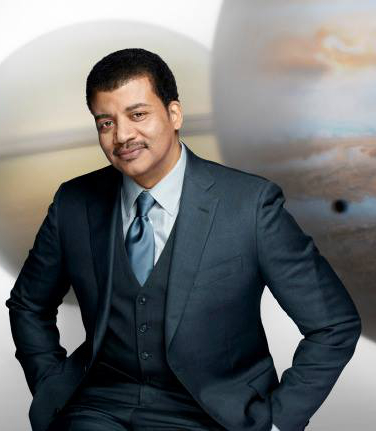
\includegraphics[width=\textwidth]{../figs/ndgt02.jpg}};
\end{tikzpicture}
\end{columns}
\vhalf
\lfr{Image: \url{http://goo.gl/hzzFUJ}}
\end{frame}

%=====
% Main slides

\begin{ftst}
{Comparison of two means}
{Dependent populations}
Suppose the following situation: a young researcher develops an optimization algorithm (A) for a given family of problems, and wants to compare its convergence speed against a method that represents the state-of-the-art (B).
\vone
The researcher implements both methods and wants to determine whether the proposed one has a better average performance for problems of that particular kind.
\vone
The measurements are made under homogeneous conditions (same computer, same operational conditions, etc.) and the time is measured in a way that is not sensitive to other processes running in the system.
\vone
\lfr{Image: \url{http://goo.gl/xwqig9}}
\begin{tikzpicture}[remember picture,overlay]
\node[anchor=south east,yshift=-5pt,xshift=5pt] at (current page.south east)
{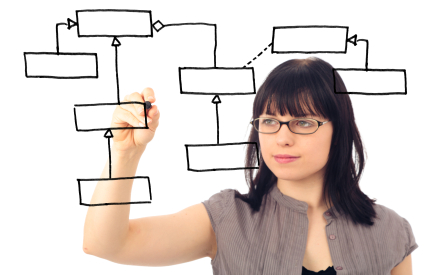
\includegraphics[width=.3\textwidth]{../figs/algoresearcher.png}};
\end{tikzpicture}
\end{ftst}

%=====

\begin{ftst}
{Comparison of two means}
{Dependent populations}
This problem has some important questions worth considering:

\bitems What is the actual question of interest?
\spitem What is the \textit{population} for which that question is relevant?
\spitem What are the independent observations for that population?
\spitem What is the relevant sample size for the experiment?
\eitem
\end{ftst}

%=====

\begin{ftst}
{Comparison of two means}
{Paired design}
The variability due to the different test problems is a strong source of spurious variation that can and must be controlled;
\vone
An elegant solution to eliminate the influence of this nuisance parameter is the \textit{pairing} of the measurements by problem:

\bitems Observations are considered in pairs (A, B) for each problem; 
\item Hypothesis testing is done on the sample of \textit{differences};
\eitem
\end{ftst}

%=====

\begin{ftst}
{Comparison of two means}
{Paired design}
Let $y_{Aj}$ and $y_{Bj}$ denote paired observations of average time for methods A and B, for each problem instance $j$. The \textit{paired differences} of the observations are simply $d_j = y_{Aj} - y_{Bj}$.
\vone
If we model our observations as an additive process:
\beqs
y_{ij} = \underbrace{\mu + \tau_i}_{\mu_i} + \beta_j + \varepsilon_{ij}
\eqs
\noindent where $\mu$ is the grand mean, $\tau_i$ is the effect of the $i$-th algorithm on the mean, $\beta_j$ is the effect of the $j$-th problem, and $\varepsilon_{ij}$ is the model residual, then:
\beqs
\begin{split}
d_j &= \cancelto{0}{\left(\mu +\beta_j - \mu - \beta_j\right)} + \tau_A-\tau_B + \varepsilon_{Aj}-\varepsilon_{Bj}\\
&=\mu_{D} + \varepsilon_j\\
\end{split}
\eqs
\end{ftst}

%=====

\begin{ftst}
{Comparison of two means}
{Paired design}
The hypotheses of interest can now be defined in terms of $\mu_D$, e.g.:
\beqs\begin{cases}
H_0: \mu_D = 0\\
H_1: \mu_D \neq 0
\end{cases}\eqs
\noindent which can now be treated as a test of hypotheses for a single sample: the population of interest is the differences in average times until convergence for the problems under investigation.
\end{ftst}

%=====

\begin{ftst}
{Comparison of two means}
{Paired design}
Some other important questions worth considering:

\bitems In this example the minimally interesting effect size $\delta^*$ must be expressed in terms of \textit{average time gains across problems} (not within individual instances);
\spitem The most important sample size to consider in this situation refers to the \textit{number of problem instances}, and not necessarily to the number of within-problems repeated measures;
\spitem The number of repetitions within each problem will have an impact on the uncertainty associated to each observation (that is, to each value of mean time to convergence for each algorithm on each problem), and should be selected with some care\footnote[2]{\tiny Alternatively, we can set it as arbitrarily large, particularly in cases where the cost of repetitions is small. As much as I hate to admit it, the lazy heuristic of setting it as $\geq 30$ should be enough in most algorithmic studies. A more methodologically sound approach to setting this is under development, and will be included in future versions of these lecture notes.}.
\eitem
\end{ftst}








%=====

\begin{ftst}
{Bibliography}
{\ }
\scriptsize
\textbf{Required reading}

\benums 
\item J.P. Simmons, L.D. Nelson, and U. Simonsohn, \textit{False-Positive Psychology : Undisclosed Flexibility in Data Collection and Analysis Allows Presenting Anything as Significant}, Psychological Science 22(11):1359-1366, 2011 - \url{http://goo.gl/9e0cdw}
\eenum

\textbf{Recommended reading}

\benums L. Lehe and V. Powell, \textit{Simpson's Paradox} - \url{http://vudlab.com/simpsons/} 
\eenum
\end{ftst}

%=====

\begin{ftstf}{About this material}{Conditions of use and referencing}
\centering\footnotesize This work is licensed under the Creative Commons CC BY-NC-SA 4.0 license\\(Attribution Non-Commercial Share Alike International License version 4.0).\\
\vhalf
\url{http://creativecommons.org/licenses/by-nc-sa/4.0/}\\
\vone
\footnotesize Please reference this work as:\\
\footnotesize \flushleft Felipe Campelo (2015), \textit{Lecture Notes on Design and Analysis of Experiments}.\\Online: {\scriptsize\url{https://github.com/fcampelo/Design-and-Analysis-of-Experiments}}\\
Version 2.11, Chapter 6; Creative Commons BY-NC-SA 4.0.\\

\begin{Verbatim}[fontsize=\tiny]
    @Misc{Campelo2015-01,
      title={Lecture Notes on Design and Analysis of Experiments},
      author={Felipe Campelo},
      howPublished={\url{https://github.com/fcampelo/Design-and-Analysis-of-Experiments}},
      year={2015},
      note={Version 2.11, Chapter 6; Creative Commons BY-NC-SA 4.0.},
    }
\end{Verbatim}

\begin{tikzpicture} [remember picture,overlay]
\node[anchor=south,yshift=0pt] at (current page.south){ \includegraphics[width=.2\textwidth]{../figs/CCSomerights.png}};
\end{tikzpicture}
\end{ftstf}


\end{document}